\documentclass[a4paper,11pt, twocolumn]{article}
\usepackage[margin=0.8in]{geometry}
\usepackage{xcolor}
\usepackage{graphicx} %package to manage images
\graphicspath{ {./images/} }
\usepackage{fancyvrb}

\title{1.3.2 Databases}
\author{Revision sheet}
\date{}

\usepackage{fancyhdr}
\pagestyle{fancy}
\fancyhead{} % clear all header fields
\renewcommand{\headrulewidth}{0pt} % no line in header area
\fancyfoot{} % clear all footer fields
\renewcommand{\footrulewidth}{0.4pt}
\fancyfoot[C]{\thepage} % page number in "outer" position of footer line
\fancyfoot[R]{\footnotesize Thomas Boxall} % other info in "inner" position of footer line
\fancyfoot[L]{\footnotesize 1.3.2 Databases \\ Revision sheet}


\begin{document}

\maketitle
\thispagestyle{fancy}

\section{Entities}
Data storage and processing is fundamental to basically every computer system. System designers have to think about how they are going to store their data and what data they will store. Generally, they will do this by listing all the entities which they will need to store. An entity is a category of object, person, event or thing which data will need to recorded about. Entities have attributes; using the example of a entity called 'Person', it might have the attributes \verb|firstName|, \verb|lastName|, \verb|phoneNumber| etc.

\section{Flat File Databases}
A flat file database consists of a single file. it might be suitable for smaller applications, like storing data of members at a local youth group. Fundamentally, it stores information about one entity. Using the example of a local youth group, you might also want to record who the parents are, these are a different entity, so you'd then have one entity of members and another of parents. This is where flat file databases aren't great - at storing more than one entity.

\section{Relational databases}
In a relational database, a separate table is created for each entity identified in the system. A number of keys are used to manage the data.
\subsection{Keys}
Keys are used in relational databases to manage the relationships between the data. There are a number of key types
\subsubsection{Primary Keys}
This is a unique identifier for a single record (entry) in a database. Quite often, a numeric or string ID is used. In the entity description, the primary key is underlined.
\subsubsection{Secondary Key}
There are a few different ways in which a database could be searched. It could be searched by looping through all the primary keys until the record which you wanted was found however this is extremely time consuming, especially in bigger databases. A secondary key is much more useful.
\subsubsection{Foreign Key}
A foreign key is an attribute that creates a join between two tables. It is the attribute that is common to both tables. The foreign key has to be a primary key in one table.
\subsection{Relationships Between Entities}
Different entities in a database may be linked in some way, if this is the case, the two entities are said to be 'related'. There are three different types of relationship between entities
\begin{itemize}
    \item \textbf{One-to-one} This is where there only can be one of each entity. For example, husband to wife.
    \item \textbf{One-to-many} This is where there can be one of one type of entity and many of the other. For example, one mother to many children (and vice versa many children to one mother).
    \item \textbf{Many-to-many} This is where there can be many of one type of entity and many of the other. For example many students to many courses.
\end{itemize}
\subsubsection{Entity-relationship diagram}
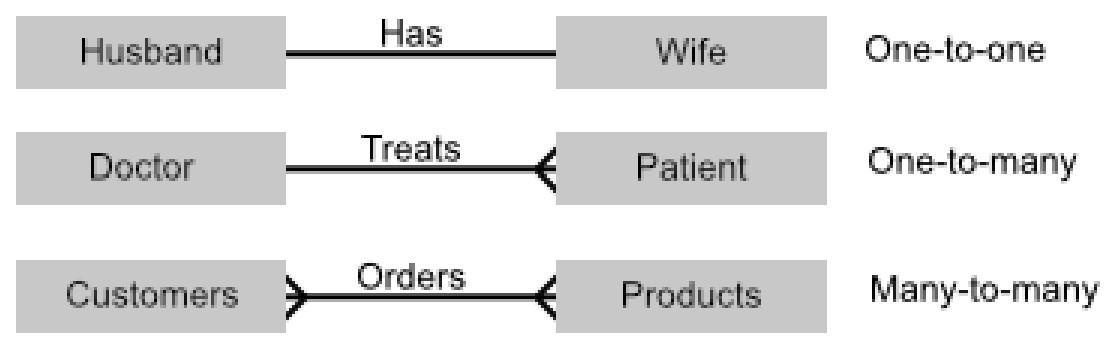
\includegraphics[width=0.45\textwidth]{images/entityRelationship.jpg}
The relationship between entities can be modelled using a diagram, with the relationships shown as seen above. 
\subsubsection{Many-To-Many relationships}
These are bad. To fix it, include a third table in between them. The only two attributes in the table should be the primary keys of the many-to-many tables. These  two primary keys will form a composite primary key.
\subsection{Referential Integrity}
When tables are linked in a relational database, it is important that when a record is deleted from one table, if an attribute is linked to another table, the records are deleted. This is called referential integrity.

\subsection{Defining a relational database}
To describe a table which has the following attributes: \verb|BookID|, \verb|DeweyCode|, \verb|Title|, \verb|Author|, \verb|DatePublished| you would need to use the following declaration:
\begin{Verbatim}[commandchars=+\[\]]
Book( +underline[BookID], DeweyCode, Title, Author, 
DatePublished)
\end{Verbatim}
The entity name is show outside the brackets, the attributes are listed within the brackets and the primary key is underlined. 

\section{Normalisation}
Normalisation is a process which is used to come up with the best possible design for a relational database. After normalisation, tables should be organised in a way such that:
\begin{itemize}
    \item no data is duplicated
    \item data is consistent throughout the database (this should be an automatic consequence of not holding duplicated data)
    \item the structure of each table is flexible enough to allow you to enter as many or few items as required
    \item the structure should enable a user to make complex queries relating data from different tables
\end{itemize}
\subsection{First normal form (1NF)}
A table is in 1NF if it contains no repeating attributes or groups of attributes. 
\subsection{Second normal form (2NF)}
A table is in 2NF if it is in 1NF and contains no partial dependencies. A partial dependency would mean that one or more of the attributes depends on only part of the primary key, which can only occur if the primary key is a composite key.
\subsection{Third normal form (3NF)}
A table is in 3NF if it is in 2NF and contains no 'non-key dependencies'. A non-key dependency is one where the value of the attribute is determined by the value of another attribute which is not part of the key. 3NF means that \textit{All attributes are dependent on the key, the whole key and nothing but the key}.
\subsection{The importance of Normalisation}
A normalised database is simply better than a un-normalised one. There is no data redundancy; it is easier to maintain and modify the database (this will also maintain data integrity); it is faster to sort and search the database and it also prevents accidental deletion of records.

\section{SQL}
\textit{See separate SQL Document.}

\section{Transaction Processing}
This is the idea that making sure any logical operations or change in state of a database (transaction) conforms to ACID for reliable processing.
\subsection{Capturing Data}
Before data can be added to a database, it has to be captured. This could either be done via manual input from data which has been captured on the high street or via a digital capture methods, one example of which is magnetic ink character recognition.
\subsection{Selecting and Managing data}
Data may have to be filtered before it can be added to a database, for example, a car speed camera may automatically photograph only those vehicles which are exceeding the speed limit. Once the data has entered the database, SQL might be used to display specific data which matches a specific criteria. Using this data, other systems might automatically be triggered, for example, sending emails.
\subsection{Exchanging Data}
A common method of transferring data between one computer system and another (usually by the internet and without the need for human intervention) is EDI (Electronic Data Interchange). This uses standardised message formatting, so documents can be exchanged electronically. Transaction software processes the transaction. EDI can be used in many different applications.
\subsection{ACID}
In the world of databases, a single logical operation on data is defined as a transaction. These transactions can be made up of many more micro steps. For example, a user buying tickets for a cinema and making an online payment is a single transaction even though it involves numerous steps. The database has to ensure that it is not possible to complete only part of a transaction, for example, booking cinema tickets without paying for it. ACID is a set of properties that guarantees that transactions are processed reliably.
\subsubsection{Atomicity}
This requires that the transaction is processed in its entirety or not at all. This includes not processing part of the transaction if there is a power cut or hard disk crashes.
\subsubsection{Consistency}
This ensures that no transaction can violate any of the defined validation rules for maintaining the integrity of the database. This links to maintaining the referential integrity of the database.
\subsubsection{Isolation}
This ensures that concurrent execution of transactions lead to the same results as if the transactions were processed one after the other.
\subsubsection{Durability}
This ensures that once a transaction has been started, it is completed. It is usually done by holding the changes needed to be made on a 'buffer disk' until all the sub-steps have been completed; only then the changes to the database will be made. 
\subsection{Problems with Multi-User Databases}
Allowing multiple people to simultaneously update a database table may cause one of the updates to be lost, unless measures are taken to prevent this. 
\subsubsection{Record Lock}
This is a technique used to prevent simultaneous access to objects in a database in order to prevent updates being lost of inconsistencies in the data arising. There is one big problem with record locking; deadlock. This is where one user is accessing person a's record and needs to access person b's record while a second user is accessing person b's record and needs to access person a's record. When this occurs the DBMS must recognise it and take action. There are a number of methods which can be used to overcome deadlock.
\subsection{Ways to avoid Deadlock}
\subsubsection{Serialisation}
This is a technique which ensures that transactions do not overlap in time therefore cannot interfere with each other or lead to updates being lost. A transaction cannot start until the previous one has finished. It can be implemented using timestamp ordering.
\subsubsection{Timestamp Ordering}
When a transaction starts, it is given a timestamp. This means if two objects affect the same object, the transaction with the earlier timestamp should be applied first. To prevent loss of transactions, every object in the database has read and write timestamps which are updated whenever the database is read or written to respectively. 
\subsubsection{Commitment ordering}
This is fundamentally the same as serialisation however it also takes note of the two transactions effect on each other.
\subsubsection{Redundancy}
Many large organisations who couldn't afford to loose moments of data if the systems went down for even a fraction of a second. Due to this, large companies will generally have copies of their data in multiple geographical locations. This builds in hardware redundency and off-site backups.


\end{document}
